\documentclass[12pt,a4paper]{article}
\usepackage[utf8]{inputenc}
\usepackage[T1]{fontenc}
\usepackage[polish]{polski}
\usepackage{amsmath}
\usepackage{amsfonts}
\usepackage{amssymb}
\usepackage{booktabs}
\usepackage{geometry}
\usepackage{enumitem}
\usepackage{graphicx}
\usepackage{float}

\geometry{margin=2cm}

\title{Systemy czasu rzeczywistego, Projekt 3}
\author{Piotr Gugnowski, wydział EiTI, nr indeksu 320690}
\date{18 Maj 2026}

\pagestyle{empty}

\begin{document}

\maketitle

\section*{Zadanie 2A — Pomiar czasów transmisji na wirtualnym porcie szeregowym}

\subsection*{Cel zadania}

Określenie możliwości zastosowania systemu operacyjnego do realizacji zadania
komunikacyjnego w czasie rzeczywistym. Poszukiwanie rozwiązań praktycznych.

\textbf{Uwaga:} Zadanie realizowane na systemie macOS zamiast Windows.

\subsection*{Parametry transmisji}

\begin{itemize}
    \item Baudrate: 115200 bps
    \item Format ramki: 8E1 (8 bitów danych, bit parzystości, 1 bit stopu)
    \item Wysyłany bajt: \texttt{0xC4}
    \item Wirtualny port szeregowy: para PTY tworzona przez \texttt{socat}
\end{itemize}

\textbf{Parametry teoretyczne:}
\begin{align*}
T_b &= \frac{1}{115200} \approx 8{,}68\ \mu\text{s} \quad \text{(czas bitu)} \\
T_{znak} &= 11 \cdot T_b \approx 95{,}49\ \mu\text{s} \quad \text{(1 start + 8 data + 1 parzystość + 1 stop)} \\
T_{gap\_max} &= 1{,}5 \cdot T_{znak} \approx 143{,}23\ \mu\text{s} \quad \text{(limit MODBUS RTU)}
\end{align*}

We wszystkich podpunktach tryb blokowy opierał się na bloku wielkości 10.
Liczba próbek w każdym pomiarze: $N = 10^6 - 1$.

% ─── a) ──────────────────────────────────────────────────────────────────────

\subsection*{a) Pomiar przy zamkniętych aplikacjach}

\subsubsection*{Treść zadania}

Napisać aplikację wysyłającą w sposób ciągły na wirtualny port szeregowy bajt \texttt{0xC4}
z parametrami 115200, 8E1. Dokonać pomiaru odstępów czasowych między wysyłaniem
kolejnych bajtów (metoda indywidualna oraz metoda blokowa). Sporządzić histogram
częstości empirycznych czasów transmisji jednego znaku. Przed uruchomieniem zamknąć
wszystkie aktywne aplikacje.

\subsubsection*{Rozwiązanie}

Aplikacja została zaimplementowana w języku Python.
Kod źródłowy dostępny jest w pliku \texttt{zadanie2a.py}.

Zastosowano dwie metody pomiaru:
\begin{itemize}
    \item \textbf{Metoda indywidualna} — każdy bajt wysyłany osobno przez \texttt{write(1B) + flush()};
          mierzony jest czas między kolejnymi wywołaniami.
    \item \textbf{Metoda blokowa} — blok $n = 10$ bajtów wysyłany jednorazowo;
          mierzony jest łączny czas bloku, a następnie dzielony przez $n$
          w celu wyznaczenia średniego czasu na bajt.
\end{itemize}

\begin{figure}[H]
    \centering
    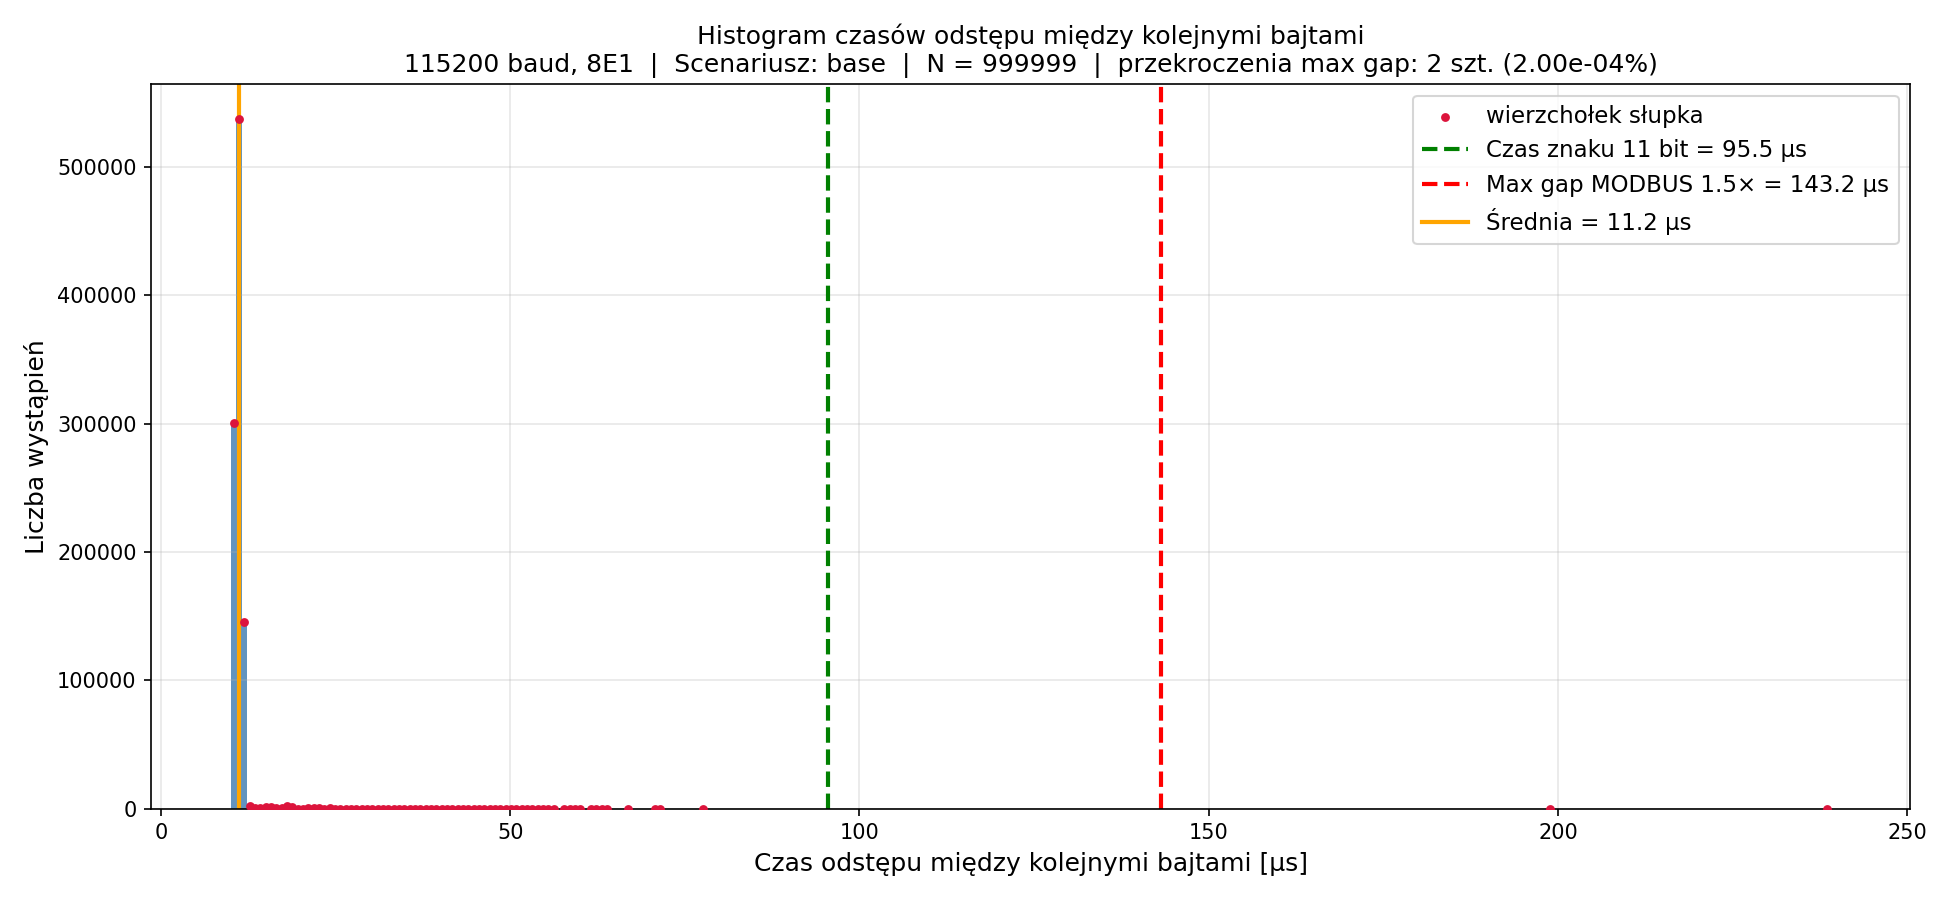
\includegraphics[width=\textwidth]{histogram_base.png}
    \caption{Histogram czasów transmisji — metoda indywidualna, aplikacje zamknięte.
             Średni czas: $\bar{t} = 11{,}2\ \mu\text{s}$, przekroczenia limitu MODBUS: 2.}
\end{figure}

\begin{figure}[H]
    \centering
    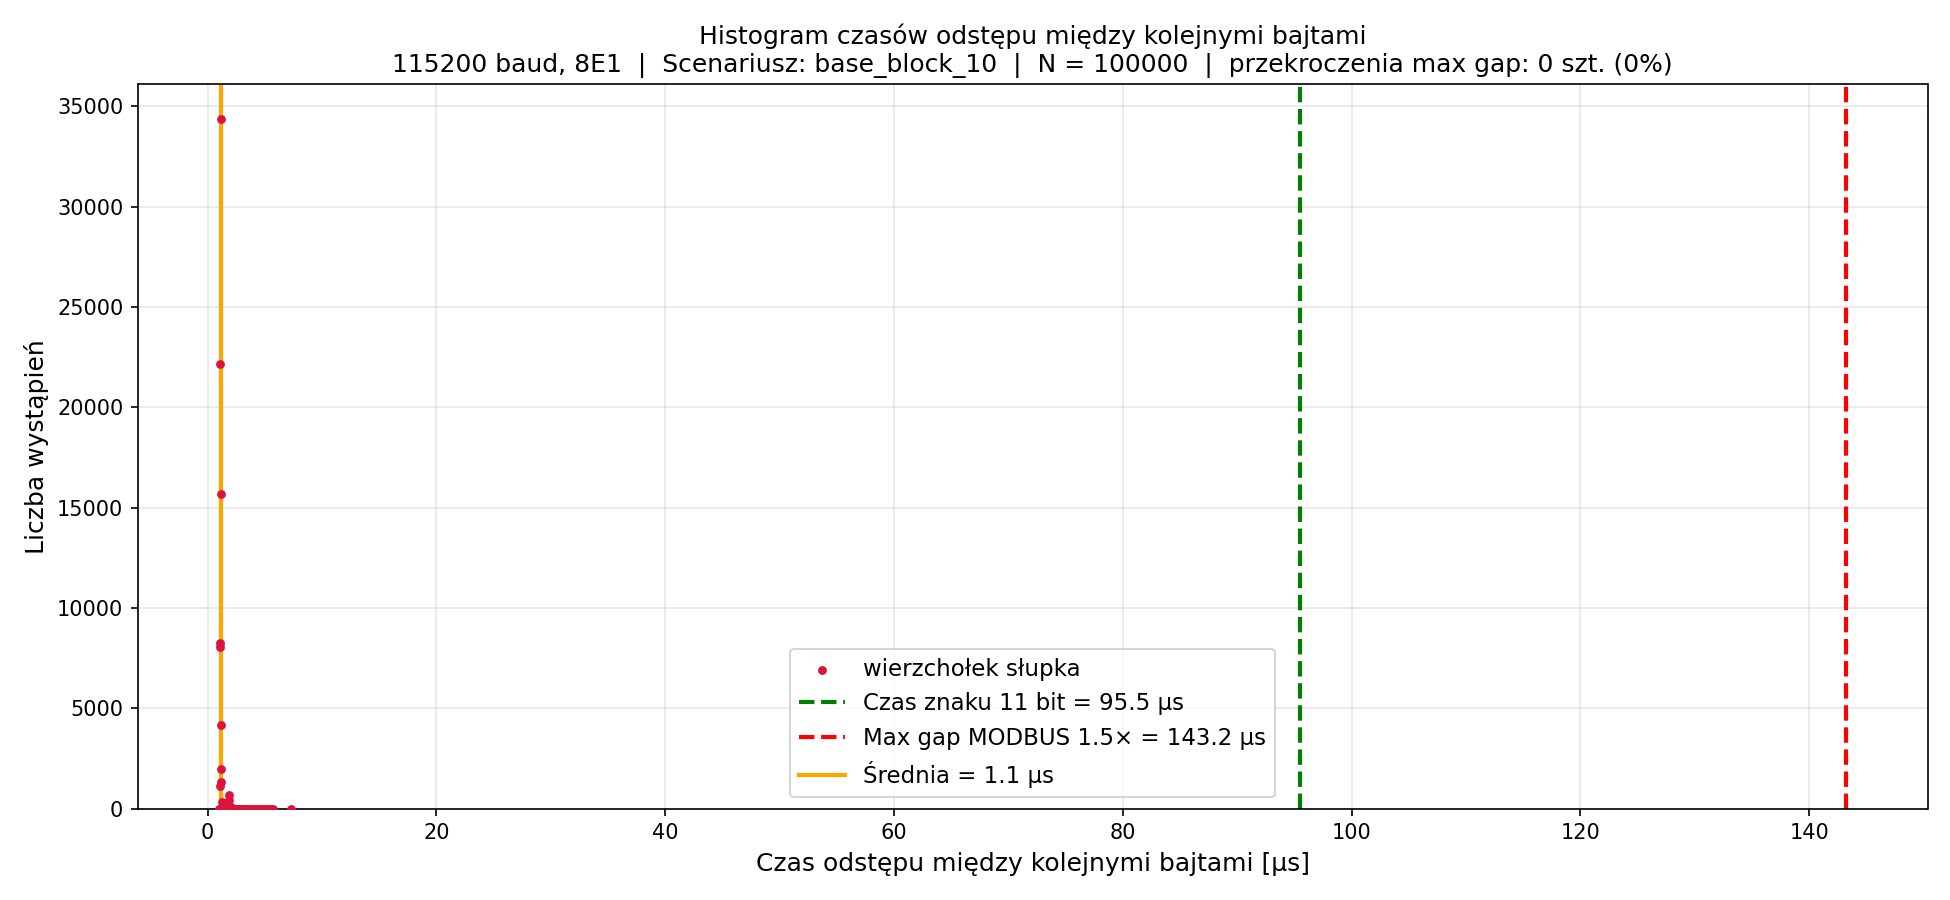
\includegraphics[width=\textwidth]{histogram_base_block_10.png}
    \caption{Histogram czasów transmisji — metoda blokowa (blok = 10 B), aplikacje zamknięte.
             Średni czas: $\bar{t} = 1{,}1\ \mu\text{s}$, przekroczenia limitu MODBUS: 0.}
\end{figure}

Średni czas w metodzie indywidualnej ($11{,}2\ \mu\text{s}$) jest niemal dziesięciokrotnie
wyższy niż w metodzie blokowej ($1{,}1\ \mu\text{s}$). Różnica wynika z~narzutu wywołań
systemowych: w metodzie indywidualnej każdy bajt generuje osobną parę wywołań
\texttt{write}/\texttt{tcdrain}, podczas gdy w metodzie blokowej ten narzut jest
amortyzowany przez $n$ bajtów. Na wirtualnym porcie (PTY) nie występuje rzeczywiste
opóźnienie sprzętowe UART, więc dominuje narzut programowy OS.
Oba wyniki są znacznie poniżej teoretycznego czasu znaku ($95{,}49\ \mu\text{s}$),
co potwierdza brak fizycznej transmisji.

% ─── b) ──────────────────────────────────────────────────────────────────────

\subsection*{b) Pomiar przy 10 aktywnych aplikacjach}

\subsubsection*{Treść zadania}

Wyznaczyć rozkład czasu transmisji przy aktywnych 10 aplikacjach.
Czy średni czas transmisji 1 znaku ulegnie zmianie?

\subsubsection*{Rozwiązanie}

Uruchomiono 10 aplikacji na komputerze i powtórzono oba pomiary.

\begin{figure}[H]
    \centering
    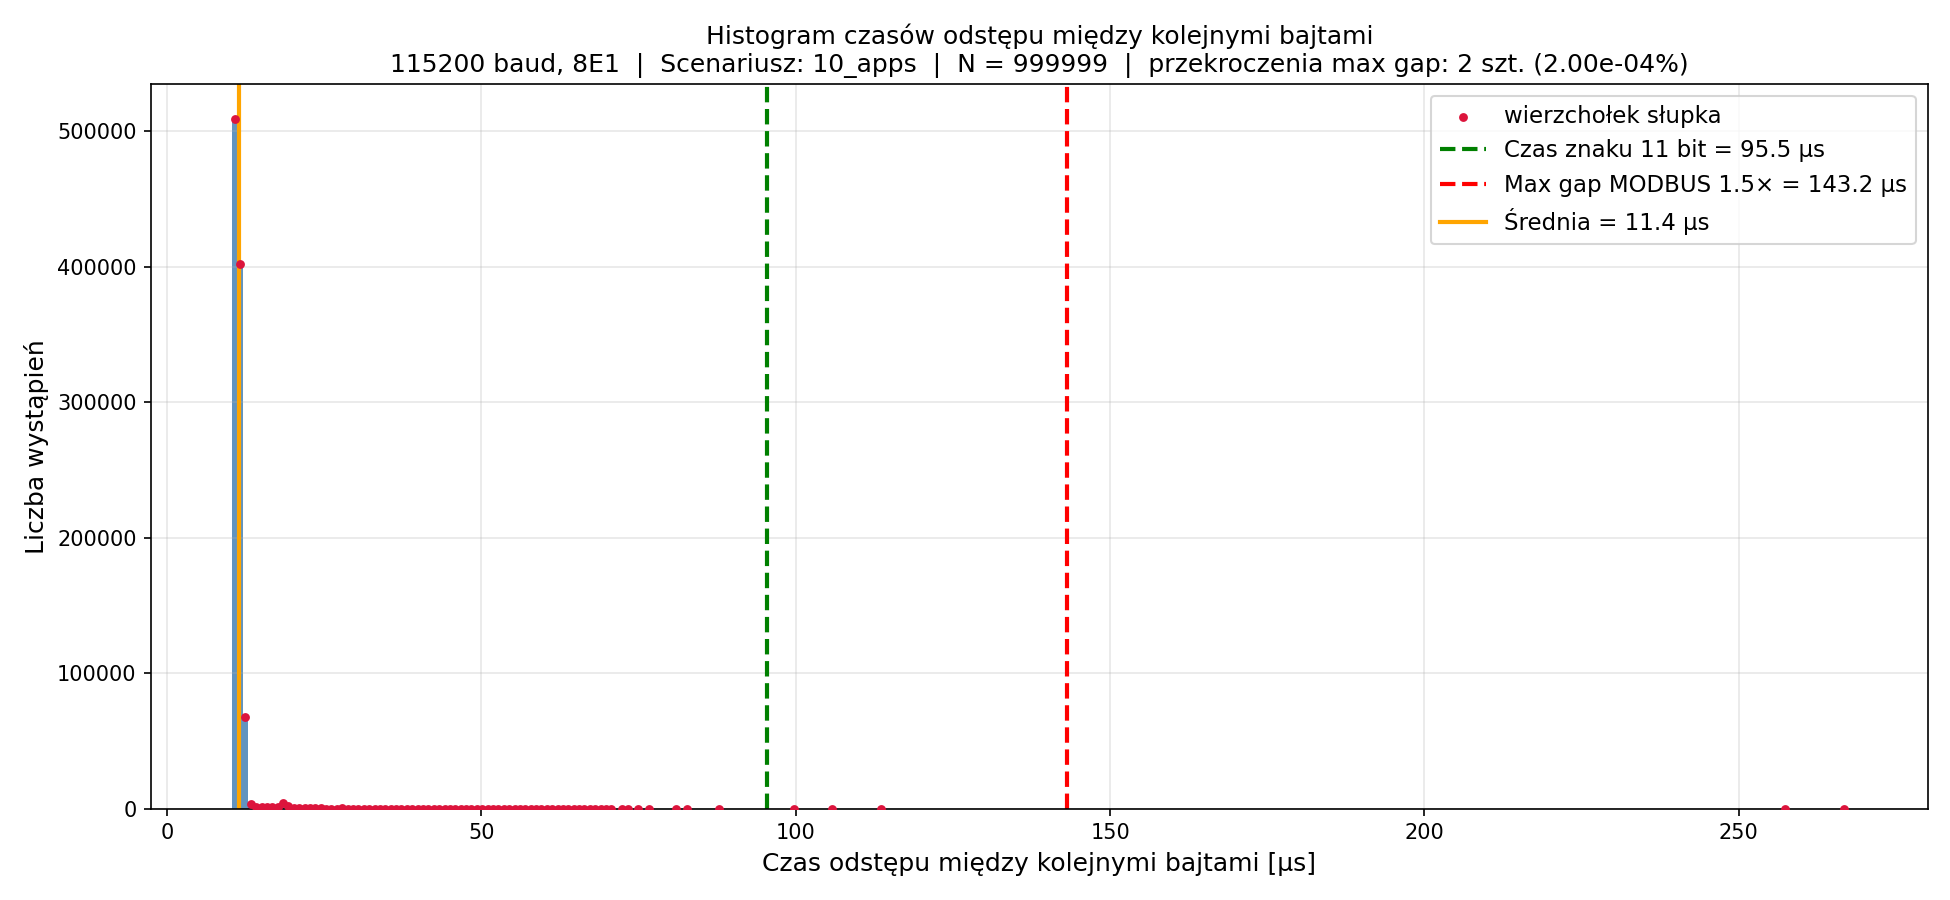
\includegraphics[width=\textwidth]{histogram_10_apps.png}
    \caption{Histogram czasów transmisji — metoda indywidualna, 10 aktywnych aplikacji.
             Średni czas: $\bar{t} = 11{,}4\ \mu\text{s}$, przekroczenia limitu MODBUS: 2.}
\end{figure}

\begin{figure}[H]
    \centering
    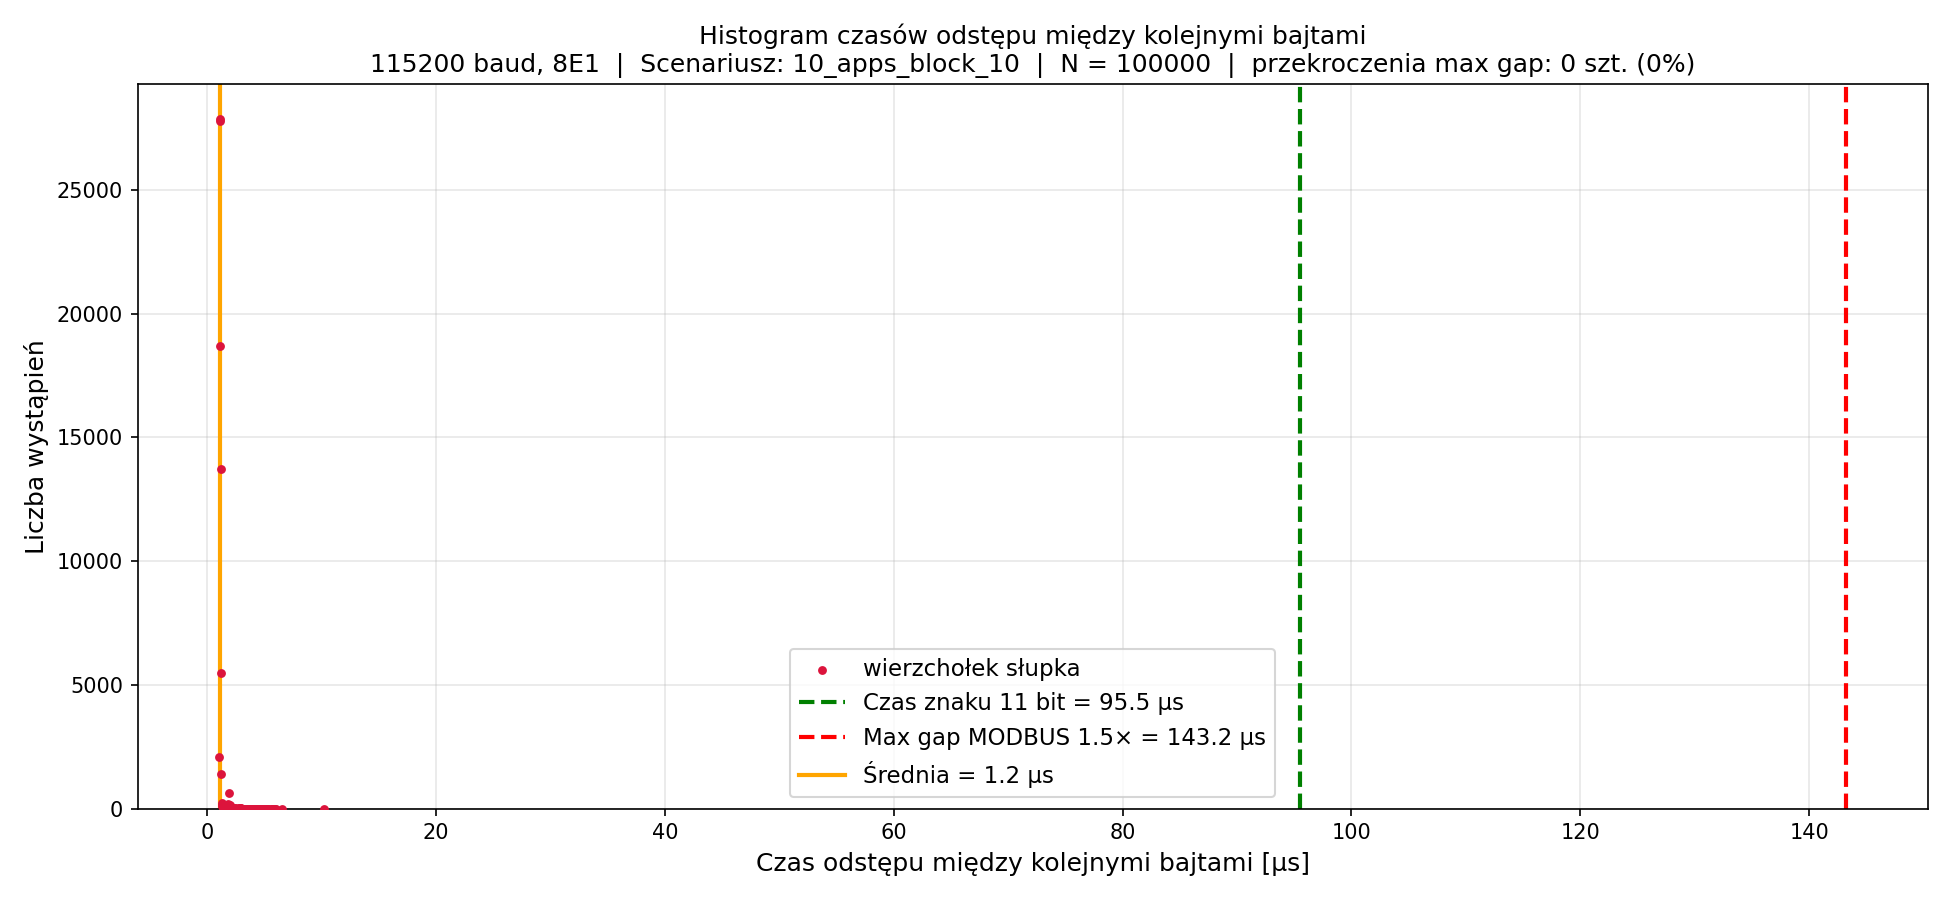
\includegraphics[width=\textwidth]{histogram_10_apps_block_10.png}
    \caption{Histogram czasów transmisji — metoda blokowa (blok = 10 B), 10 aktywnych aplikacji.
             Średni czas: $\bar{t} = 1{,}2\ \mu\text{s}$, przekroczenia limitu MODBUS: 0.}
\end{figure}

Średni czas transmisji uległ zmianie w obu przypadkach:
\begin{itemize}
    \item metoda indywidualna: $11{,}2 \to 11{,}4\ \mu\text{s}$ (wzrost o~$\approx 1{,}8\%$),
    \item metoda blokowa: $1{,}1 \to 1{,}2\ \mu\text{s}$ (wzrost o~$\approx 9\%$).
\end{itemize}
Aktywne aplikacje zwiększają obciążenie schedulera, co przekłada się na większy
jitter i nieznacznie wyższy średni czas między wysyłanymi bajtami.
Liczba przekroczeń limitu MODBUS nie zmieniła się (2 w metodzie indywidualnej),
co sugeruje, że wzrost obciążenia na poziomie 10 aplikacji jest jeszcze
niewystarczający, by istotnie pogorszyć terminowość transmisji.

% ─── c) ──────────────────────────────────────────────────────────────────────

\subsection*{c) Wpływ operacji na oknach}

\subsubsection*{Treść zadania}

Zbadać wpływ operacji na oknach (ręczne przeciąganie i skalowanie okien) na
średni czas transmisji 1 znaku.

\subsubsection*{Rozwiązanie}

Podczas pomiaru wykonywano intensywne operacje na oknach systemu
(przeciąganie, skalowanie).

\begin{figure}[H]
    \centering
    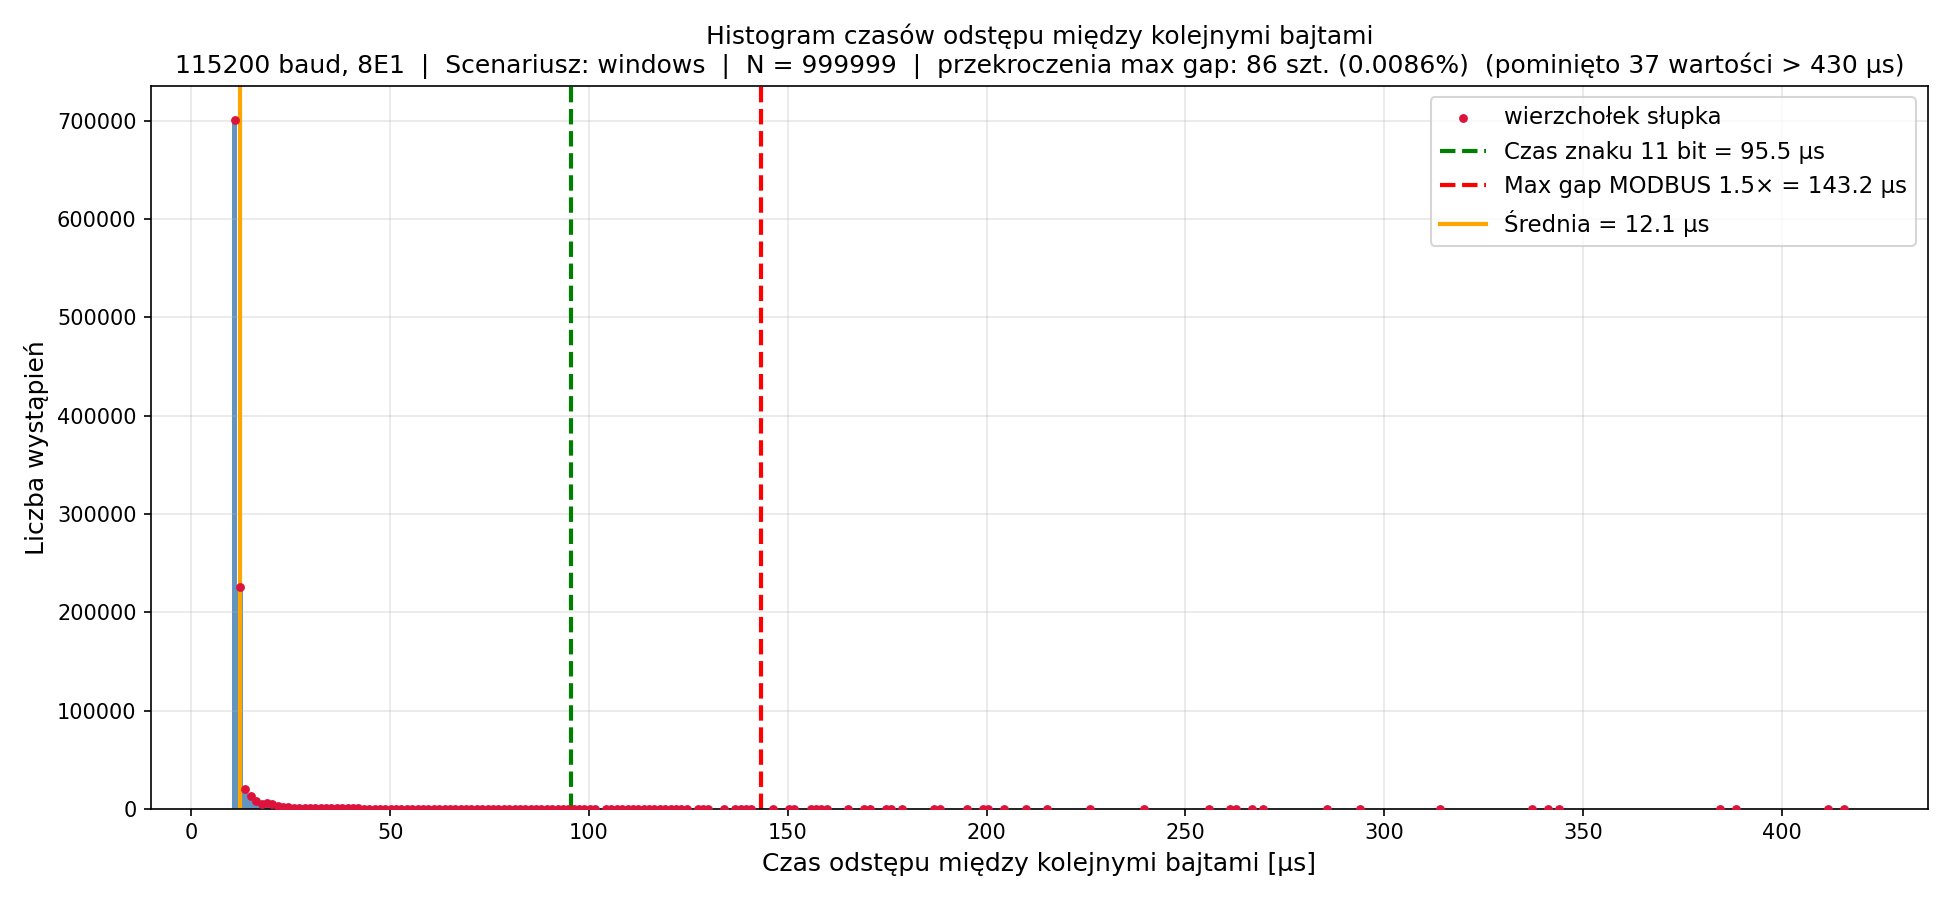
\includegraphics[width=\textwidth]{histogram_windows.png}
    \caption{Histogram czasów transmisji — metoda indywidualna, operacje na oknach.
             Średni czas: $\bar{t} = 12{,}1\ \mu\text{s}$, przekroczenia limitu MODBUS: 86.}
\end{figure}

\begin{figure}[H]
    \centering
    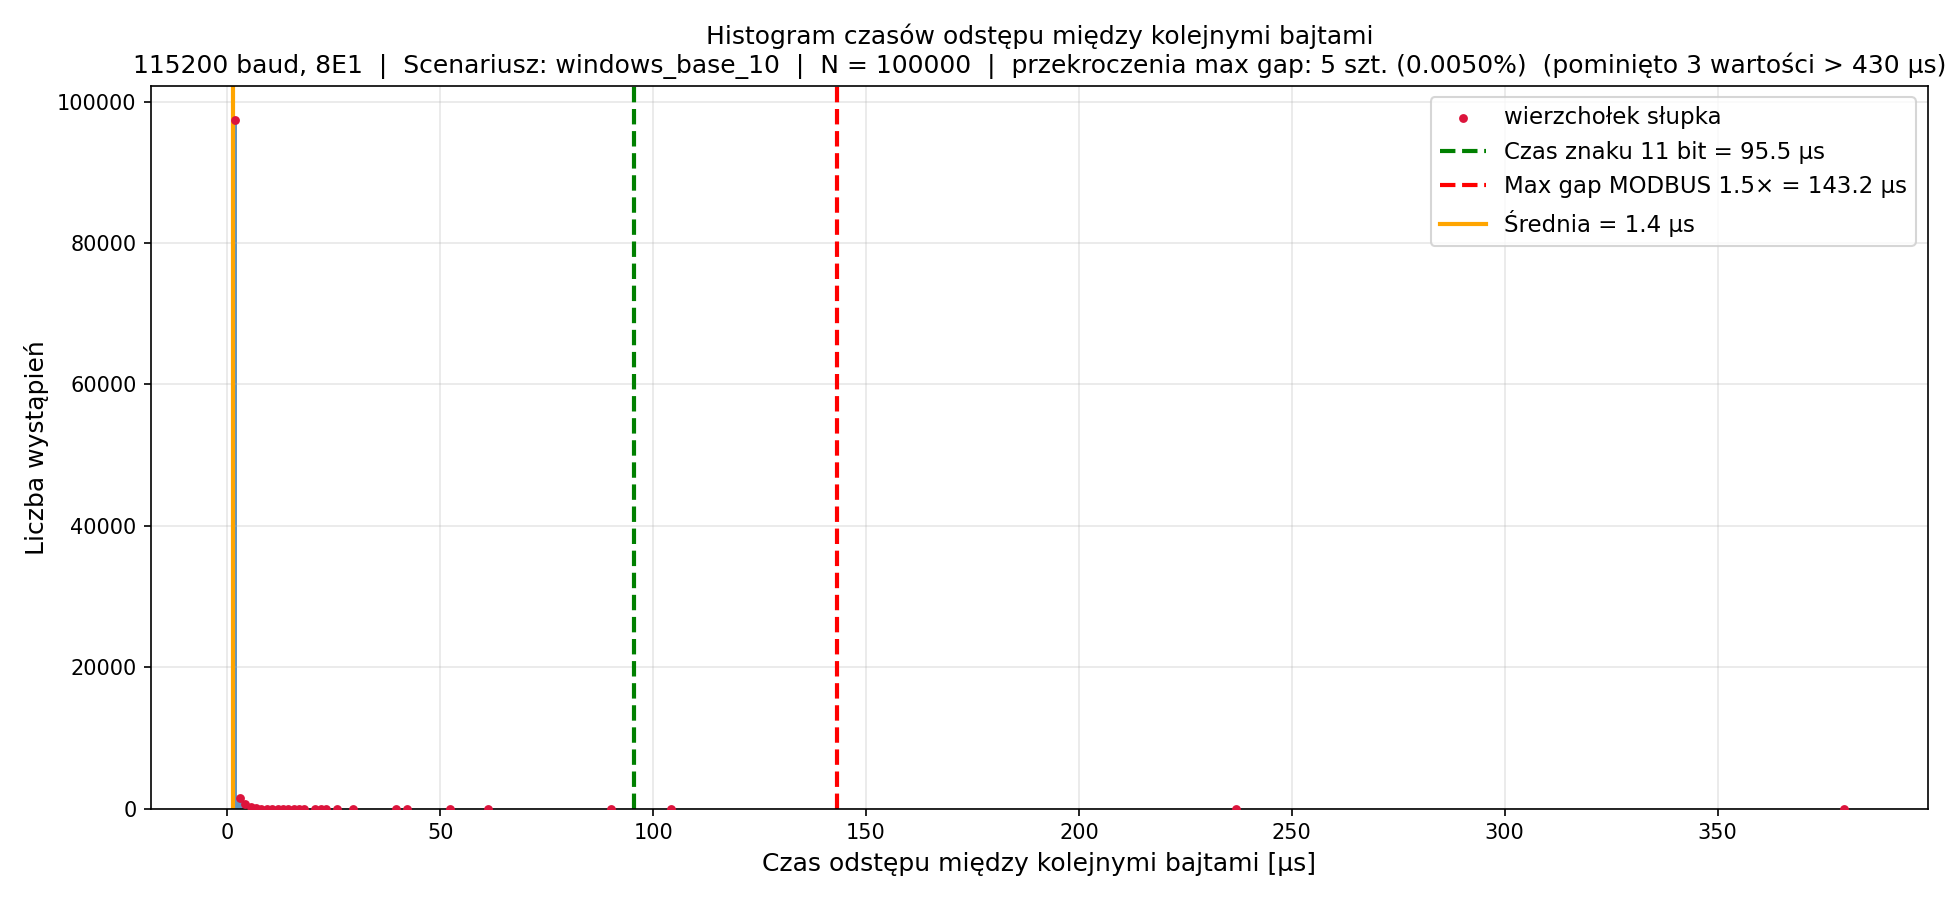
\includegraphics[width=\textwidth]{histogram_windows_base_10.png}
    \caption{Histogram czasów transmisji — metoda blokowa (blok = 10 B), operacje na oknach.
             Średni czas: $\bar{t} = 1{,}4\ \mu\text{s}$, przekroczenia limitu MODBUS: 5.}
\end{figure}

Operacje na oknach spowodowały wyraźne pogorszenie parametrów transmisji:
\begin{itemize}
    \item metoda indywidualna: średni czas wzrósł o~$\approx 8\%$
          ($11{,}2 \to 12{,}1\ \mu\text{s}$), liczba przekroczeń wzrosła z 2 do \textbf{86},
    \item metoda blokowa: średni czas wzrósł o~$\approx 27\%$
          ($1{,}1 \to 1{,}4\ \mu\text{s}$), pojawiło się \textbf{5} przekroczeń
          (wcześniej: 0).
\end{itemize}
Poruszanie oknami angażuje podsystem graficzny (GPU, compositor), co powoduje
długie wywłaszczenia procesu pomiarowego przez system operacyjny.
Skutkuje to gwałtownym wzrostem liczby przekroczeń limitu MODBUS RTU,
szczególnie widocznym w metodzie blokowej — tryb blokowy nie zapewnia tu
żadnej ochrony przed nieregularnościami schedulera.

System macOS, podobnie jak Windows, jest systemem operacyjnym ogólnego
przeznaczenia (GPOS) i nie gwarantuje deterministycznych czasów odpowiedzi.
Operacje graficzne znacząco obniżają terminowość transmisji szeregowej.
W zastosowaniach hard real-time wymagany byłby dedykowany system czasu
rzeczywistego (RTOS) lub sprzętowe wsparcie dla priorytetyzacji zadań czasowych.

% ═══════════════════════════════════════════════════════════════════════════
\section*{Zadanie 2B — Pomiar odstępów między znakami w ramce MODBUS RTU}
% ═══════════════════════════════════════════════════════════════════════════

\subsection*{Cel zadania}

Zbadanie rozkładu czasów odstępów między kolejnymi znakami w ramce protokołu
MODBUS RTU, przy różnych obciążeniach systemu operacyjnego.

\textbf{Uwaga:} Zadanie realizowane na systemie macOS zamiast Windows.

\subsection*{Parametry transmisji}

\begin{itemize}
    \item Baudrate: 115200 bps, format 8E1
    \item Wysyłana ramka: \texttt{01 03 00 00 00 02 C4 0B} (8 znaków)
    \item Metoda: wyłącznie zastępcza — $\bar{T}_{znak} = T_{ramka} / 8$
    \item Liczba ramek w każdym pomiarze: $N = 10^6 - 1$
\end{itemize}

\textbf{Parametry teoretyczne:}
\begin{align*}
T_{znak}     &\approx 95{,}49\ \mu\text{s} \qquad \text{(minimum: 11 bitów × }T_b\text{)} \\
T_{ramka}    &= 8 \cdot T_{znak} \approx 763{,}89\ \mu\text{s} \qquad \text{(minimum teoretyczne)} \\
T_{gap\_max} &= 1{,}5 \cdot T_{znak} \approx 143{,}23\ \mu\text{s} \qquad \text{(limit MODBUS RTU)}
\end{align*}

% ─── 2B a) ───────────────────────────────────────────────────────────────────

\subsection*{a) Pomiar przy zamkniętych aplikacjach}

\subsubsection*{Treść zadania}

Dokonać pomiaru rozkładu czasów odstępu pomiędzy kolejnymi znakami w ramce
metodą zastępczą. Sporządzić histogram częstości empirycznych.
Przed uruchomieniem zamknąć wszystkie aktywne aplikacje.

\subsubsection*{Rozwiązanie}

\begin{figure}[H]
    \centering
    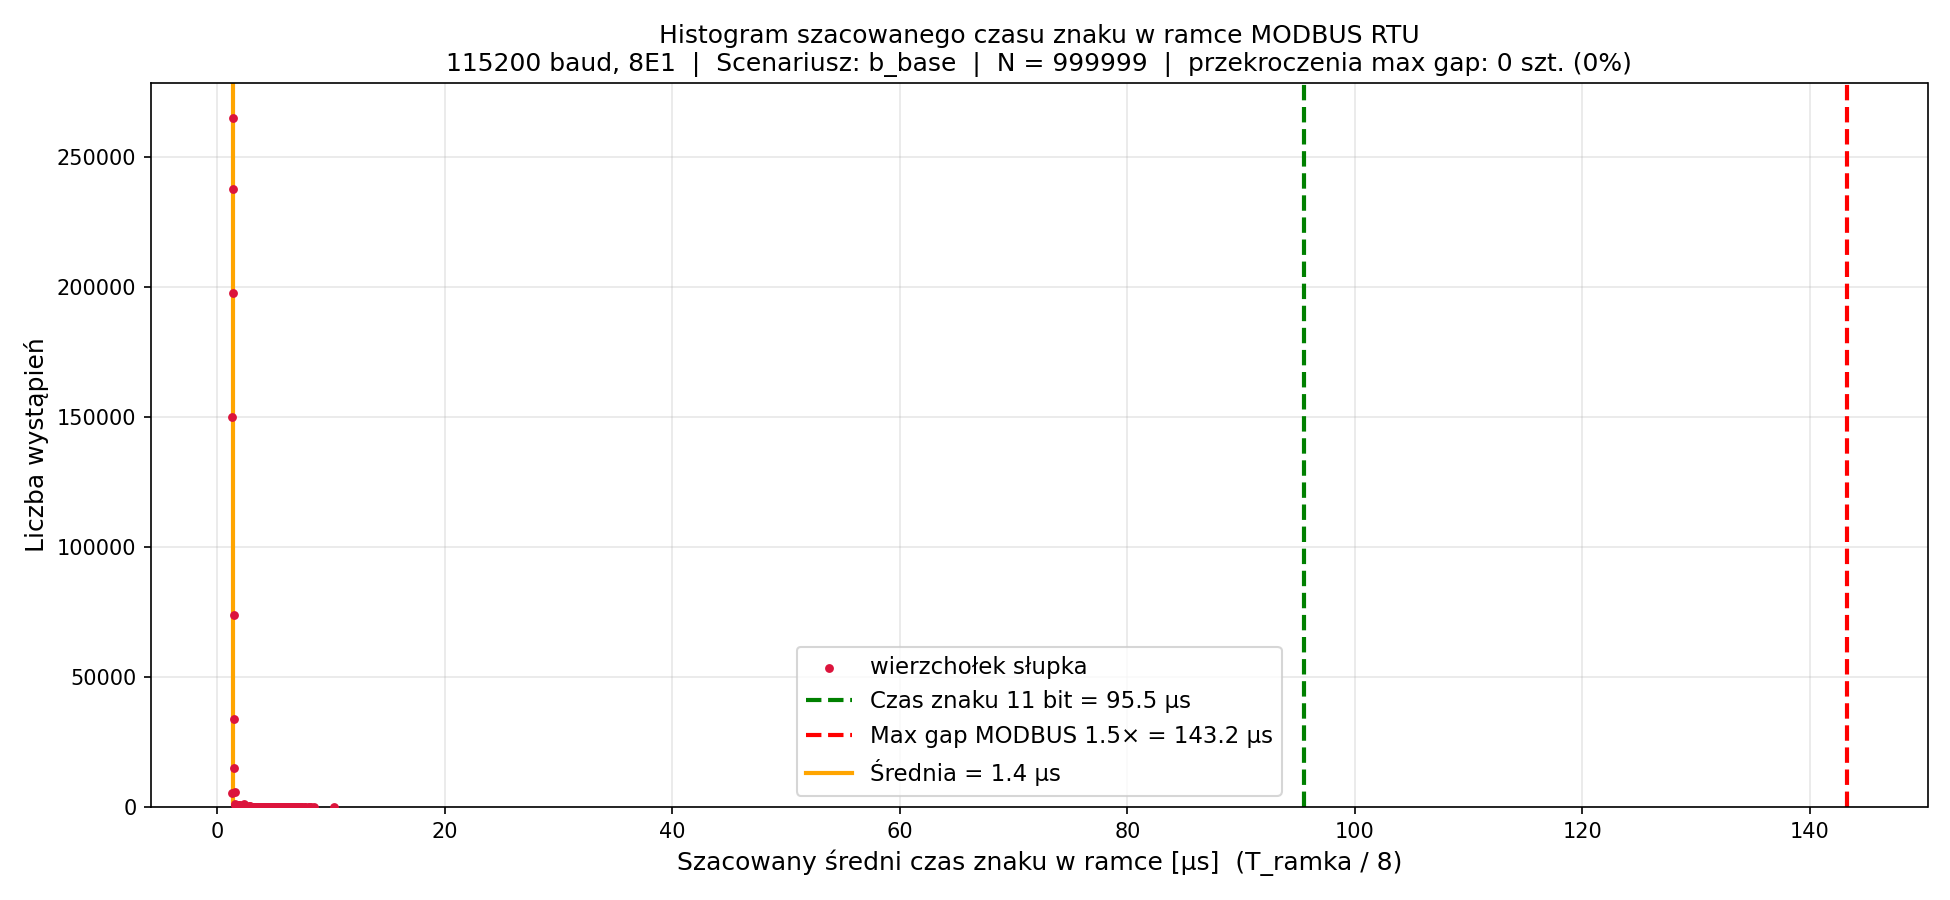
\includegraphics[width=\textwidth]{histogram_b_base.png}
    \caption{Histogram szacowanego czasu znaku w ramce MODBUS RTU — aplikacje
             zamknięte. Średni czas: $\bar{T}_{znak} = 1{,}4\ \mu\text{s}$,
             przekroczenia limitu MODBUS: 0.}
\end{figure}

Szacowany średni czas znaku wynosi $1{,}4\ \mu\text{s}$, co jest znacznie poniżej
wartości teoretycznej $T_{znak} \approx 95{,}49\ \mu\text{s}$. Wynika to z~faktu,
że pomiar odbywa się na wirtualnym porcie PTY, gdzie nie występuje rzeczywiste
opóźnienie sprzętowego UART — czas mierzony to wyłącznie narzut programowy OS
na wysłanie 8~bajtów. Nie odnotowano żadnych przekroczeń limitu MODBUS RTU,
co oznacza, że w~stanie spoczynku systemu ramka jest wysyłana płynnie i~bez
przerw wywłaszczeniowych.

% ─── 2B b) ───────────────────────────────────────────────────────────────────

\subsection*{b) Pomiar przy 10 aktywnych aplikacjach}

\subsubsection*{Treść zadania}

Wyznaczyć rozkład czasów odstępów przy aktywnych 10 aplikacjach.
Czy średni czas transmisji 1~znaku ulegnie zmianie?

\subsubsection*{Rozwiązanie}

Uruchomiono 10 aplikacji na komputerze i~powtórzono pomiar.

\begin{figure}[H]
    \centering
    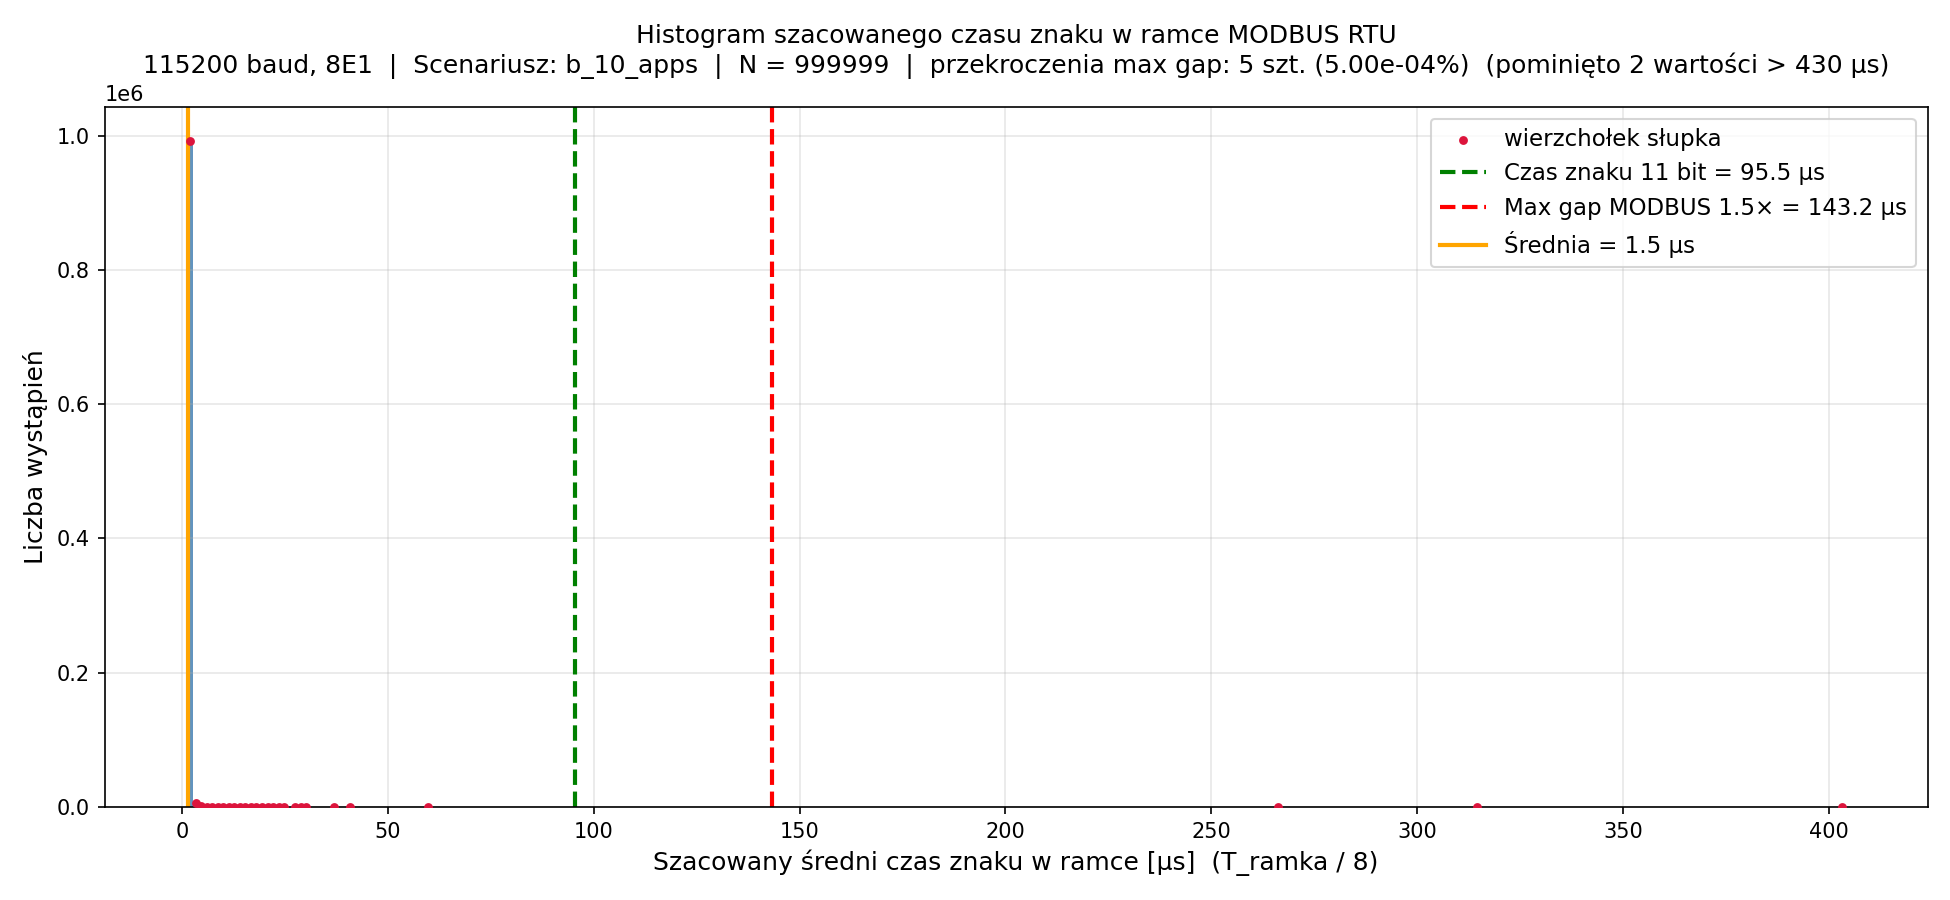
\includegraphics[width=\textwidth]{histogram_b_10_apps.png}
    \caption{Histogram szacowanego czasu znaku w ramce MODBUS RTU — 10 aktywnych
             aplikacji. Średni czas: $\bar{T}_{znak} = 1{,}5\ \mu\text{s}$,
             przekroczenia limitu MODBUS: 5.}
\end{figure}

Aktywne aplikacje spowodowały wzrost średniego czasu o~$\approx 7{,}1\%$
($1{,}4 \to 1{,}5\ \mu\text{s}$). Pojawiło się 5~przekroczeń limitu MODBUS RTU
(wcześniej: 0) — scheduler obciążony 10~procesami wywłaszcza sporadycznie
proces pomiarowy podczas wysyłania ramki, co wprowadza przerwy rzędu setek mikrosekund.

% ─── 2B c) ───────────────────────────────────────────────────────────────────

\subsection*{c) Wpływ operacji na oknach}

\subsubsection*{Treść zadania}

Zbadać wpływ ręcznego przeciągania i~skalowania okien na średni czas odstępu
między znakami w~ramce.

\subsubsection*{Rozwiązanie}

Podczas pomiaru wykonywano intensywne operacje na oknach systemu.

\begin{figure}[H]
    \centering
    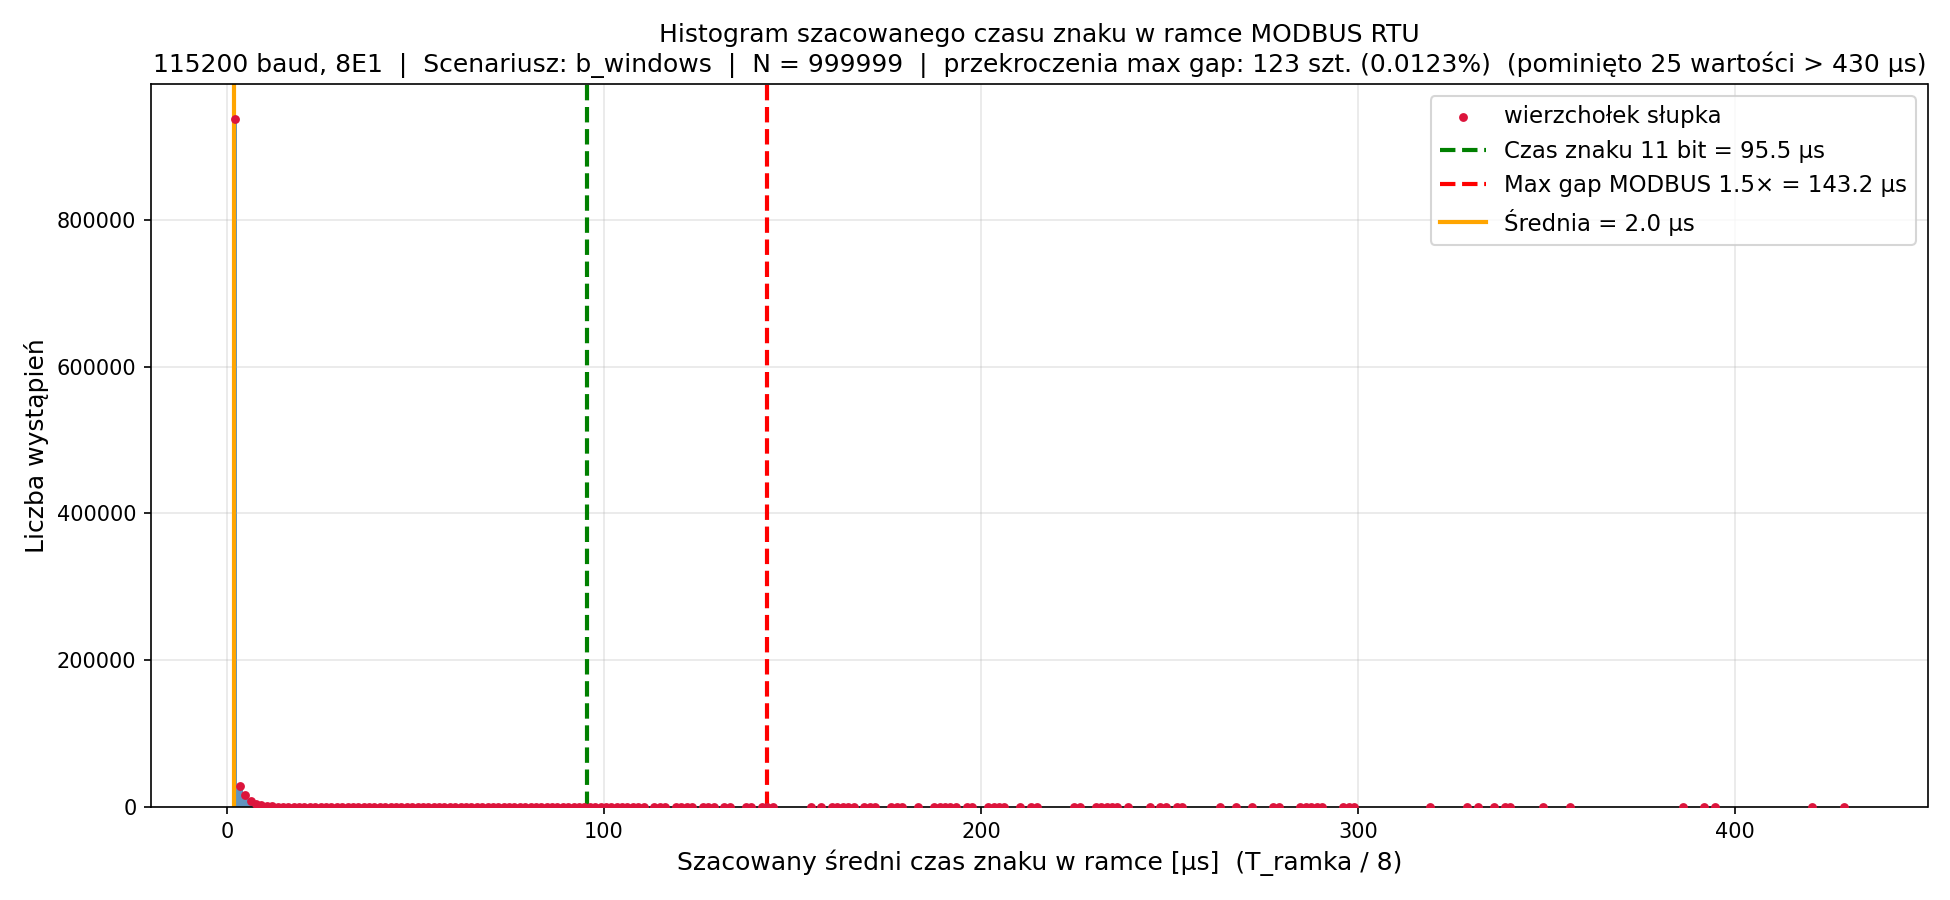
\includegraphics[width=\textwidth]{histogram_b_windows.png}
    \caption{Histogram szacowanego czasu znaku w ramce MODBUS RTU — operacje
             na oknach. Średni czas: $\bar{T}_{znak} = 2{,}0\ \mu\text{s}$,
             przekroczenia limitu MODBUS: 123.}
\end{figure}

Operacje na oknach spowodowały gwałtowne pogorszenie parametrów:
\begin{itemize}
    \item Średni czas wzrósł o~$\approx 42{,}9\%$ względem wartości bazowej
          ($1{,}4 \to 2{,}0\ \mu\text{s}$).
    \item Liczba przekroczeń limitu MODBUS RTU wzrosła do \textbf{123}
          (z~0 w~stanie bazowym i~5 przy 10~aplikacjach).
\end{itemize}
Przeciąganie okien angażuje compositor okienkowy i~sterownik GPU, co powoduje
długotrwałe wywłaszczenia procesu pomiarowego. Dla protokołu MODBUS RTU jest to
krytyczne — każde z~123 przekroczeń odpowiada przerwie $> 143{,}23\ \mu\text{s}$
w~środku ramki, co odbiorca zinterpretowałby jako koniec transmisji i~odebrał
ramkę jako niekompletną lub błędną.

W zadaniu 2A metoda zastępcza (blok 10~bajtów) dała 5~przekroczeń podczas
operacji na oknach, podczas gdy 2B (ramka 8~bajtów) dała 123.
Bezpośrednie porównanie tych liczb jest jednak mylące — w~obu przypadkach
poruszano innymi aplikacjami: w~2A przesuwano okno edytora VSCode, natomiast
w~2B okno komunikatora Discord. Discord jest aplikacją znacznie bardziej
obciążającą GPU i~compositor (renderowanie interfejsu webowego na Electron),
co powoduje dłuższe i~częstsze wywłaszczenia procesu pomiarowego.
Wyniki potwierdzają tym samym, że rodzaj aplikacji działającej w~tle
ma istotny wpływ na determinizm czasowy transmisji.

System macOS, jako GPOS, nie gwarantuje terminowego wysyłania ramek MODBUS RTU
przy obciążeniu systemu. Operacje graficzne powodują przekroczenia limitu
inter-character gap, co w~rzeczywistej instalacji przemysłowej oznaczałoby
utratę spójności komunikacji. Aplikacje krytyczne czasowo wymagają RTOS
lub dedykowanego sprzętowego kontrolera komunikacyjnego.

% ─── Implementacja ───────────────────────────────────────────────────────────

\subsection*{Implementacja}

Do realizacji pomiarów napisano dwa skrypty w języku Python, współdzielące
wspólną bibliotekę \texttt{shared.py} zawierającą stałe transmisji
($T_b$, $T_{znak}$, $T_{gap\_max}$) oraz funkcje statystyczne i wizualizacyjne.

\textbf{zadanie2a.py} realizuje transmisję ciągłą bajtu \texttt{0xC4}.
Dostępne są dwie metody pomiaru: metoda indywidualna, w której każdy bajt
wysyłany jest osobno przez wywołanie \texttt{write(1B) + flush()}, a czas
między kolejnymi wywołaniami jest mierzony jako odstęp; oraz metoda blokowa
(zastępcza), w której blok $n$ bajtów wysyłany jest jednorazowo, a zmierzony
czas całkowity dzielony jest przez $n$ w celu uzyskania średniego czasu na bajt.
Wyniki wizualizowane są jako histogram z liniami referencyjnymi $T_{znak}$
i $T_{gap\_max}$. Skrypt przyjmuje parametry przez CLI: port, liczba próbek,
etykieta scenariusza, wybór metody oraz katalog wyjściowy.

\textbf{zadanie2b.py} realizuje transmisję ciągłą ramki MODBUS RTU
\texttt{01 03 00 00 00 02 C4 0B} (8 bajtów). Stosowana jest wyłącznie metoda
zastępcza: mierzony jest czas całej ramki, który następnie dzielony jest przez
liczbę znaków ($N = 8$), co daje szacowany średni czas na znak
$\bar{T}_{znak} = T_{ramka} / 8$. Wizualizacja i CLI analogiczne do
\texttt{zadanie2a.py}; brak opcji metody blokowej.

Uruchamianie pomiarów odbywa się za pomocą skryptów powłoki
\texttt{run\_pomiar\_2a.sh} i \texttt{run\_pomiar\_2b.sh}, które automatycznie
tworzą wirtualną parę portów szeregowych przez \texttt{socat}, wykrywają
ścieżki PTY i uruchamiają drainer bufora na drugim porcie. Wspólna logika
(uruchomienie \texttt{socat}, oczekiwanie na inicjalizację portów, obsługa
\texttt{cleanup}) wydzielona jest do \texttt{shared.sh}.

% ─── Dodatek ─────────────────────────────────────────────────────────────────

\appendix
\section*{Dodatek A — Wywłaszczalność zadań}

\subsection*{Pojęcie wywłaszczalności}

Wywłaszczalność (\textit{preemptibility}) oznacza zdolność systemu operacyjnego do
przerwania aktualnie wykonywanego zadania w~dowolnym momencie i~przekazania procesora
innemu zadaniu o~wyższym priorytecie. W systemach z~wywłaszczaniem wielozadaniowym
(\textit{preemptive multitasking}) — do których należą macOS i~Windows — scheduler może
wywłaszczyć dowolny proces w~każdej chwili, niezależnie od tego, czy jest on gotowy na
takie przerwanie.

\subsection*{Wpływ na pomiary}

Każdy skok na histogramie powyżej wartości typowej jest bezpośrednim śladem
wywłaszczenia procesu pomiarowego. Sekwencja zdarzeń:

\begin{enumerate}
    \item Proces pomiarowy wywołuje \texttt{write()} i~\texttt{flush()}, po czym
          scheduler uznaje, że inne zadanie OS ma wyższy priorytet.
    \item Proces zostaje zawieszony na czas kwantu schedulera lub dłużej,
          jeśli inne zadania utrzymują wysoki priorytet.
    \item Po powrocie do wykonania proces mierzy czas — różnica zawiera całe
          opóźnienie wywłaszczenia.
\end{enumerate}

Stąd wynikają obserwacje z~pomiarów:
\begin{itemize}
    \item \textbf{Ogon prawostronny histogramu} — rzadkie, duże wartości
          odpowiadają długim wywłaszczeniom (np.\ przez podsystem graficzny).
    \item \textbf{Wzrost liczby przekroczeń limitu MODBUS z~2 do 86}
          przy operacjach na oknach — compositor i~sterownik GPU przejmują
          procesor na czas renderowania klatki.
    \item \textbf{Metoda blokowa nie eliminuje wywłaszczenia} — jeśli
          wywłaszczenie nastąpi podczas wywołania \texttt{write(block)},
          jego koszt jest jedynie $1/n$-krotnie mniejszy, nie zerowy.
\end{itemize}

\subsection*{GPOS vs.\ RTOS}

\begin{center}
\begin{tabular}{lll}
\toprule
Cecha & GPOS (macOS / Windows) & RTOS \\
\midrule
Polityka schedulera & priorytet + kwant czasu & priorytet ściśle hierarchiczny \\
Wywłaszczenie zadania RT & możliwe przez zadania OS & tylko przez wyższy priorytet \\
Maksymalne opóźnienie & nieokreślone & gwarantowane (WCET) \\
Źródło jitteru & ISR, compositor, GC, sieć & tylko przerwania wyższego priorytetu \\
\bottomrule
\end{tabular}
\end{center}

W systemie RTOS zadanie RT przypisane do odpowiedniego priorytetu nie zostałoby
wywłaszczone przez podsystem graficzny, co wyeliminowałoby prawy ogon histogramu
i~przekroczenia limitu MODBUS.

% ─── Dodatek B ────────────────────────────────────────────────────────────────

\section*{Dodatek B — Podstawy teoretyczne: Zadanie 2B}

\subsection*{Ramka MODBUS RTU}

\textit{Ramka} (ang.\ \textit{frame}) to niepodzielna sekwencja znaków
traktowana przez protokół jako jedna jednostka komunikacji. W protokole
MODBUS RTU granice ramki wyznaczane są przez ciszę na łączu dłuższą niż
$3{,}5 \times T_{znak}$ (przed ramką) i~$1{,}5 \times T_{znak}$ między
kolejnymi znakami wewnątrz ramki.

Badana ramka to zapytanie jednostki nadrzędnej o~odczyt 2 rejestrów Holding:

\begin{center}
\begin{tabular}{cll}
\toprule
Bajt(y) & Wartość (hex) & Znaczenie \\
\midrule
1   & \texttt{01}      & Adres urządzenia slave (1) \\
2   & \texttt{03}      & Kod funkcji: Read Holding Registers \\
3--4 & \texttt{00 00}  & Adres startowy rejestru (0) \\
5--6 & \texttt{00 02}  & Liczba rejestrów do odczytu (2) \\
7--8 & \texttt{C4 0B}  & Suma kontrolna CRC-16 (little-endian: \texttt{0x0BC4}) \\
\bottomrule
\end{tabular}
\end{center}

\subsection*{Znak i ramka znakowa (11 bitów)}

Każdy bajt transmitowany jest jako \textit{znak} złożony z 11 bitów na łączu (format 8E1):

$$1\ \text{(start)} + 8\ \text{(dane)} + 1\ \text{(parzystość)} + 1\ \text{(stop)} = 11\ \text{bitów}$$

\begin{align*}
T_b       &= \frac{1}{115200} \approx 8{,}68\ \mu\text{s} \\
T_{znak}  &= 11 \cdot T_b \approx 95{,}49\ \mu\text{s} \\
T_{ramka} &= 8 \cdot T_{znak} \approx 763{,}89\ \mu\text{s} \quad \text{(minimum teoretyczne)}
\end{align*}

\textit{Inter-character gap} to cisza między końcem jednego znaku a~początkiem
następnego. Limit MODBUS RTU: gap $> 1{,}5 \times T_{znak} \approx 143{,}23\ \mu\text{s}$
jest interpretowany jako koniec ramki — odbiorca uznaje transmisję za przerwaną.

\subsection*{Metoda zastępcza pomiaru}

Bezpośredni pomiar każdego odstępu wymagałby sprzętowego timestampowania
na poziomie bitu (oscyloskop lub analizator protokołów). W~ramach metody
zastępczej mierzy się czas całej ramki $T_{ramka}$ i~szacuje się średni
czas na znak:

$$\bar{T}_{znak} = \frac{T_{ramka}}{N_{znaków}} = \frac{T_{ramka}}{8}$$


\end{document}
